\scanpage{97}
Soit $u'$ le composé \deleted{$\unsure{u'_{j,n}|u'_{j,h}}$} $B\quad E_{k,n}\qquad E'_{j,n}\quad u'_{j,h}\quad D'$, où la première flêche est l'hom de transition, alors $u'$ est le relèvement cherché.

\margin{\handwritten{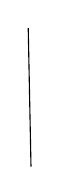
\begin{tikzpicture}[x=1em,y=1em]\draw (0,0)--(.1,-5);\end{tikzpicture}}}
Mettre le corollaire 2.2. sous forme de l'équivalence de trois conditions (i) $B$ form simple (ii) Condition 1º et 2º (iii) $\hat B$ est isomorphe comme alg top à $\hat B'$, où $B'$ est l'algèbre symmétrique d'un $C$-module projectif, munie de \deleted{\unsure{la}} sa topologie définie par son idéal d'augmentation. La forme (iii) est en effet parfois commode, et est obtenue directement dans la démonstration.

\inserted{\handwritten{(\unsure{i$'$bis|i bis}) Pour tout hom de $B$ dans $B'$ \deleted{une \unsure{Algèbre quotient|Algèbre, quotient} \unsure{de} $D'/J$, \unsure{$J$ d'indice}} considéré comme quotient d'une alg. de polynômes \unsure{tronqués}, \deleted{on peut relever \unsure{en un} \unsure{hom}} \deleted{$C[\unsure{t}]$} $B'_{\unsure{(1)|(i)}}$ où $B'_{(0)}=C$, on peut relever,}}
\margin{\handwritten{$\unsure{\text{si}|b'}\ I/I^{\unsure{2|?}}$ de type fini}}
% Left-pointing leader to the small note.

Dans la suite du paragraphe Cohen, 3.4. devient un corollaire immédiat de 3.3. grâce à 2.2. D'ailleurs 3.3. admet toute une kyrielle de corollaires qui dans ma rédaction étaient dans un odre assez chaotique, je suggère \deleted{\unsure{les|le}} l'ordre suivant:

1º Existence d'un corps de représentants dans un anneau \inserted{local noeth} complet, quand l'extension résiduelle est séparable. (Cf 3.5.)

2º (oublié dans ma rédaction). Soit $A$ anneau local nœth complet. Les conditions suivantes sont équivalentes: (i) $A$ contient un corps (ii) Si $\operatorname{car} k(A)=p\quad0$, alors $pA=0$ (iii) $A$ est isomorphe à un anneau quotient d'un anneau $k\ T_1,\ldots,T_n$ sur un corps $k$. (iv) (Si $A$ est intègre de corps des fractions $K$) $k(A)$ et $K$ ont même caractéristique . On peut se borner à donner (iv) à titre de commentaire (c'est une autre façon d'énoncer (ii) simplement), pour \deleted{\unsure{rappeler|rappelerx}} rappeler l'ancienne terminologie \textquotedblleft cas d'égale caractéristique\textquotedblright. Je suggère que nous ne suivions pas cette terminologie, car il est aussi court de \unsure{dife|dire} \textquotedblleft A contient un corps\textquotedblright, et la terminologie \textquotedblleft égale car\textquotedblright\ est fort ambigue pour des anneaux non intègres, par exemple artiniens.

% archive sheet number: 96
